
\clearpage
\refstepcounter{PagePtr}\label{P:charCode}
\section{文字コードについて}
コンピュータは数字の0,
1しかわからないことを学びました。
0,1の2種類でなる数字列を2進数(バイナリ)といいます。
ところで、文字はどのように表示されているのでしょうか?そこで使われるのが文字コードです。
コンピュータは結局\ruby{数値}{すうち}しかわからないので、数値と文字の\ruby{対応}{たいおう}を用いて、人間のわかる文字を表現します。
その対応にあたるものが文字コードで、数字列を文字に\ruby{変換}{へんかん}するルールです。

例えば、ASCIIでは英語のアルファベットをすべて表現できます。
ASCIIはアメリカで決められ、\ruby{英語圏}{えいごけん}ではよく使われます。
ASCIIのテーブルをみて、表現を確認してみましょう。


\bigskip

{\bfseries
表のDecimalは10進数の数値,
Hex(Hexadecimal)は16進数の数値,
Char(Character)は文字を意味します。}


\bigskip

[\url{https://simple.wikipedia.org/wiki/ASCII}]

\begin{center}
  % Unhandled or unsupported graphics:
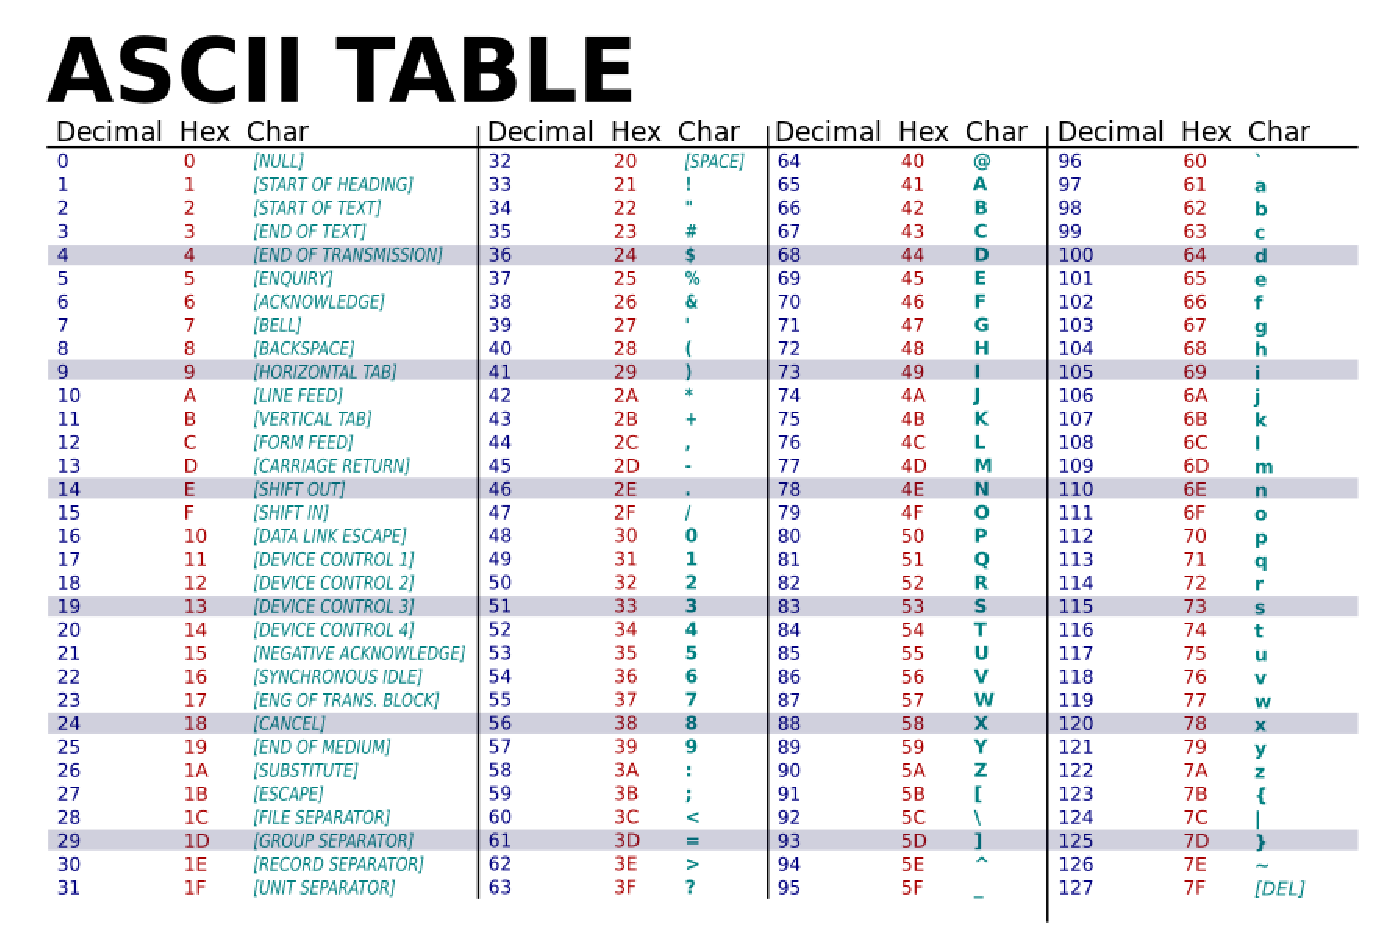
\includegraphics[width=14cm]{./text08-img/textbook-img016.eps}

\end{center}
ASCII
コードでは2進数7\ruby{桁}{けた}で一つの文字を表します。
128個の文字を表すことができます。


\bigskip


\bigskip


\bigskip

\clearpage
ASCIIでは0〜127を使用していました。
しかし、漢字などたくさんの文字がある日本語、中国語などではこの数値の\ruby{範囲}{はんい}に\ruby{収}{おさ}まりません。
いろいろな会社や\ruby{組織}{そしき}が\ruby{別々}{べつべつ}の方法で工夫して日本語を表現したので、\ruby{異}{こと}なる文字コードがあります。

代表的な文字コードと使いみちの例をあげます。

\begin{itemize}
\item Shift\_JIS \ruby{日本語版}{にほんごばん}Windows・Mac
\item EUC-JP \ruby{旧}{きゅう}UNIXワークステーション
\item ISO-2022-JP 電子メール
\item Unicode(UTF-8)
ラズベリーパイ、スマートフォン、海外版Windows


\bigskip
\end{itemize}

\bigskip
\refstepcounter{Exercise}
\clearpage\section{\theExercise 数字をASCIIを使って、ターミナルに文字を表示する}
\addtocounter{Exercise}{-1}\refstepcounter{Exercise}\label{E:ASCII}
考え方

\ \ printfコマンドを使用すると数字をASCIIに\ruby{従}{したが}って文字へ変換できます。
表のHEXの列をみて、41,
42,
43を探してみましょう。
何が表示されるか考えて試してみましょう。

ターミナルを開いて、

\ \ \textbf{printf “{\textbackslash}x41 {\textbackslash}x42 {\textbackslash}x43 {\textbackslash}n”}

を実行しましょう。

一番最後についている{\textbackslash}nは改行(カーソルを次の行に変える)という意味があります.

{\textbackslash}xはHE\textbf{X}(16進数であることを指定します)

\begin{center}
  % Unhandled or unsupported graphics:
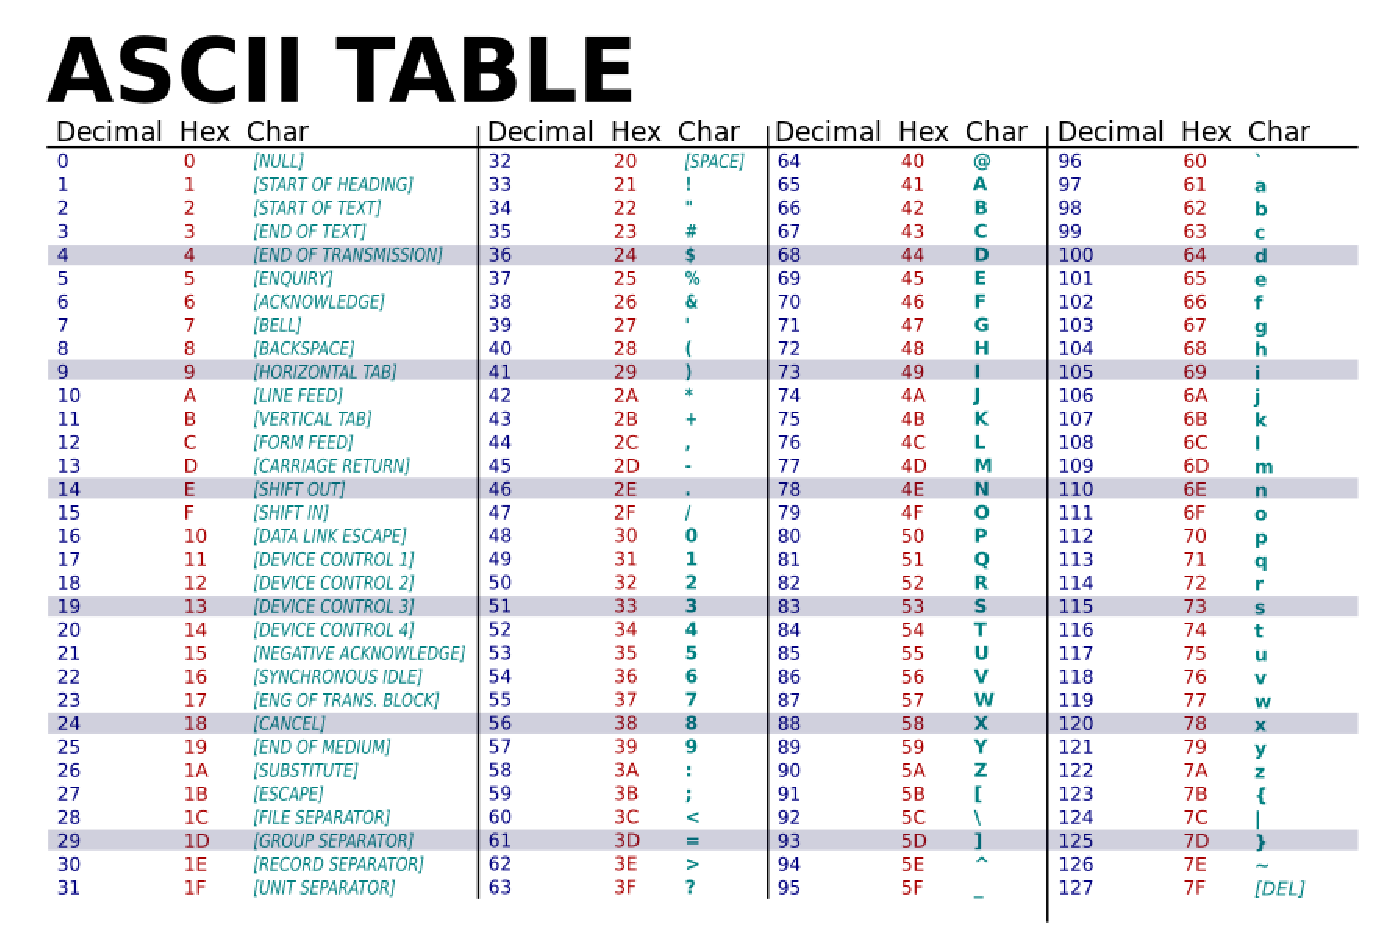
\includegraphics[width=\textwidth]{./text08-img/textbook-img016.eps}

\end{center}

\bigskip


\bigskip

{\bfseries
表のDecimalは10進数の数値,
Hex(Hexadecimal)は16進数の数値,
Char(Character)は文字を意味します。}

{\bfseries
[\url{https://simple.wikipedia.org/wiki/ASCII}]}

\refstepcounter{Question}
\clearpage\subsection*{\theQuestion\label{Q:myName}}
\begin{itemize}
\item
ASCIIを使ってローマ字で自分の名前を表示させてみよう
\end{itemize}
\refstepcounter{Question}
\subsection*{\theQuestion\label{Q:friendName}}
\begin{itemize}
\item
ASCIIを使ってローマ字でとなりの友達の名前を表示させてみよう
\end{itemize}
\refstepcounter{Question}
\subsection*{\theQuestion\label{Q:emoticon}}
\begin{itemize}
\item
ASCIIで顔文字を作って表示させてみよう
\end{itemize}
\ \ 例.) (* \^{} *) \ (* \_ *) \ (d\_b)


\bigskip

{\bfseries
表のDecimalは10進数の数値,
Hex(Hexadecimal)は16進数の数値,
Char(Character)は文字を意味します。}

\begin{center}
  % Unhandled or unsupported graphics:
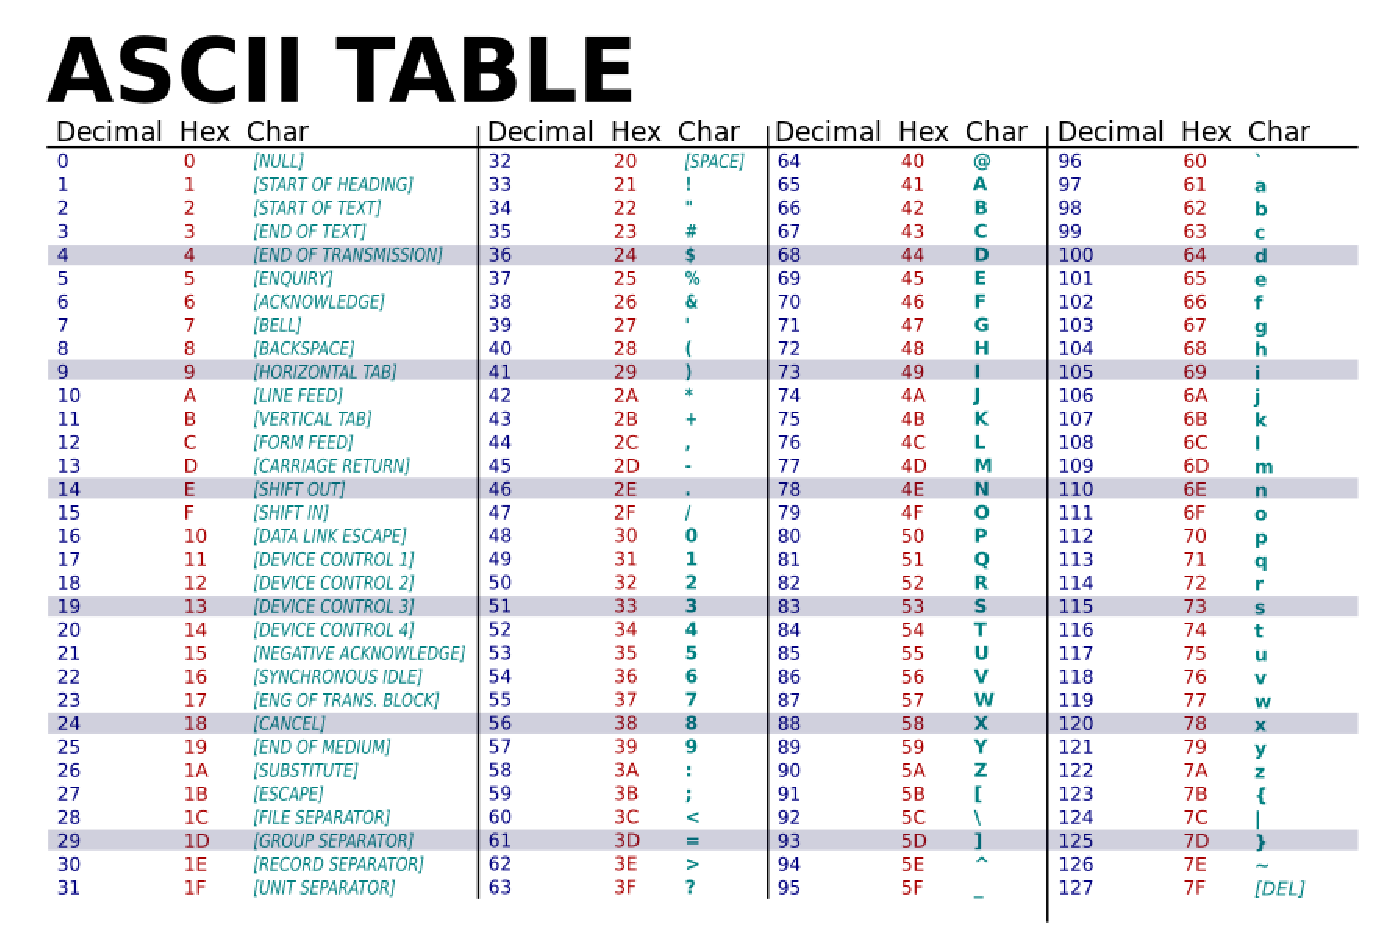
\includegraphics[width=\textwidth]{./text08-img/textbook-img016.eps}

\end{center}
{\bfseries
[\url{https://simple.wikipedia.org/wiki/ASCII}]}
\refstepcounter{Exercise}
\clearpage\section{\theExercise 数字をUTF-8を使って、ターミナルに文字を表示する}
\addtocounter{Exercise}{-1}\refstepcounter{Exercise}\label{E:UTF8}
考え方

\ \ printfコマンドを使用すると数字をUTF-8に従って文字に変換できます。
UTF-8は日本語も漢字を\ruby{含}{ふく}め表現することができます。

授業で使用したホームページを開いてください。\textbf{({\textasciitilde}/08/links.html)}



\begin{center}
  % Unhandled or unsupported graphics:
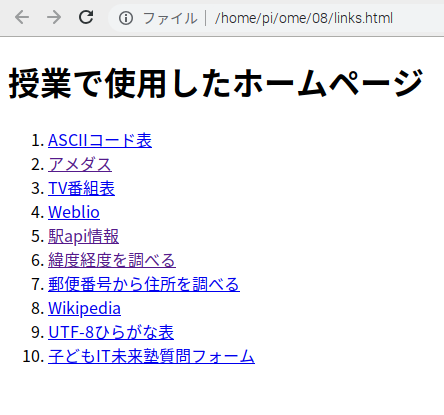
\includegraphics[width=0.6\textwidth]{./text08-img/textbook-img017.png}

\end{center}


\bigskip

9.
UTF-8ひらがな表を開いてください。
UTF-8のひらがなに対応する数値の表があります。

”あ”を表示したい場合、”あ”がある行を見るとE3
81
80となっています。
列を見ると2となっています。
これらを足すと

E3 81 80 + 2 = E3 81 82

[\url{http://orange-factory.com/sample/utf8/code3/e3.html#Hiragana}]

\begin{center}
  % Unhandled or unsupported graphics:
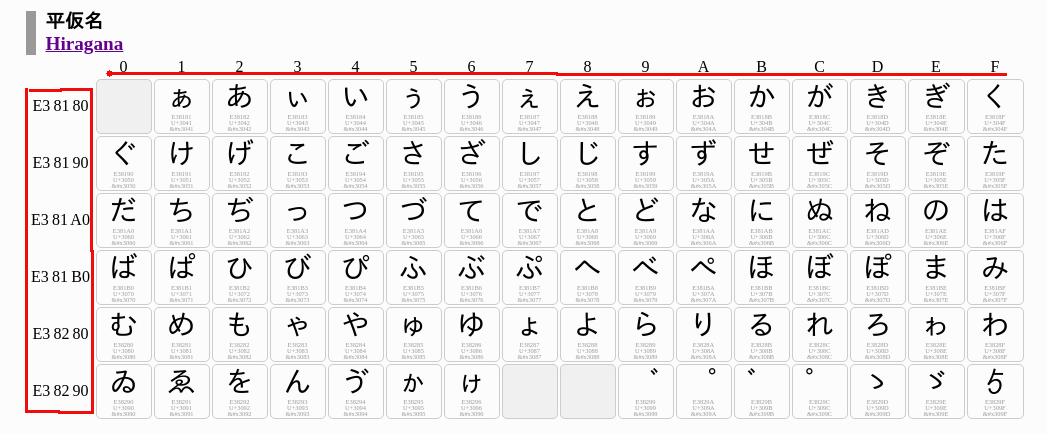
\includegraphics[width=\textwidth]{./text08-img/textbook-img018.png}

\end{center}
ターミナルを開いて、

\ \ \textbf{printf “{\textbackslash}xe3{\textbackslash}x81{\textbackslash}x82{\textbackslash}n”}

を実行しましょう。

一番最後についている{\textbackslash}nは改行(カーソルを次の行に変える)という意味があります.

{\textbackslash}xはHE\textbf{X}(16進数であることを指定します)

\refstepcounter{Question}
\subsection*{\theQuestion\label{Q:myNameUTF8}}
\begin{itemize}
\item
UTF-8を使ってひらがなで自分の名前を表示させてみよう
\end{itemize}
\refstepcounter{Question}
\subsection*{\theQuestion\label{Q:friendNameUTF8}}
\begin{itemize}
\item
UTF-8を使ってひらがなでとなりの友達の名前を表示させてみよう
\end{itemize}

\bigskip



\begin{center}
  % Unhandled or unsupported graphics:
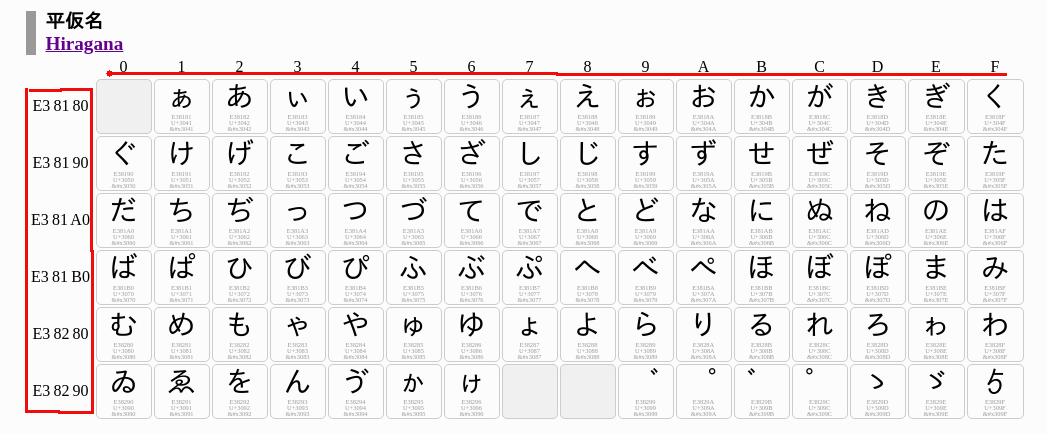
\includegraphics[width=\textwidth]{./text08-img/textbook-img018.png}

\end{center}

\bigskip

[\url{http://orange-factory.com/sample/utf8/code3/e3.html#Hiragana}]
\refstepcounter{Exercise}
% \clearpage\section{\theExercise ウェブページで使用されている文字コードを変換する}
\clearpage\section{\theExercise ウェブページをダウンロードして、表示してみよう}
\addtocounter{Exercise}{-1}\refstepcounter{Exercise}\label{E:iconv1}
考え方

ある文字コードで表現された文字列を他の文字コードで\ruby{解釈}{かいしゃく}すると文字化けをする\ruby{可能性}{かのうせい}があります。
例えば、UTF-8と\ruby{設定}{せってい}されたターミナルなどのアプリケーションでEUC-JPで書かれたファイルを開くなどすると文字化けをします。
これは、文字を表現するのに2つの文字コード間で数値が\ruby{違}{ちが}うからです。
ターミナルなどのアプリケーションから正しく\ruby{扱}{あつ}うためには、ターミナルやアプリケーションが使っている文字コードに変換する必要があります。
この例では変換の練習をします。

ターミナルが使っている文字コードを確認してみよう

echo \$LANG

% jp\_ja.UTF-8

\begin{center}
  % Unhandled or unsupported graphics:
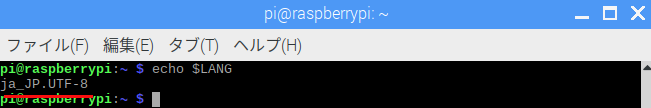
\includegraphics[width=\textwidth]{./text08-img/textbook-img019.png}



\end{center}
jp\_ja.UTF-8\\
国\_言語.文字コード

のように表されています。
ターミナルはUTF-8の文字コードを使用しています。
LANGは(\ruby{環境}{かんきょう})変数で、アプリケーションやコマンドが使用するロケール(国や\ruby{地域}{ちいき}によって異なる言語や単位、日付などの表記など)の設定をします。


LANGに設定されている文字コードと表示したい文字コードが異なっていると、文字化けをします。例えば、UTF-8を使っているシステムで、EUC-JPで表現された文字列を表示した場合など。


試しにUTF-8以外の文字コードを使用しているウェブサイトをcurlでダウンロードして、UTF-8として設定されているターミナルに表示させてみよう

\textbf{cd {\textasciitilde}/08}

curl \url{http://x68000.q-e-d.net/~68user/unix/pickup?iconv} -o hsp.html

\begin{center}
  % Unhandled or unsupported graphics:
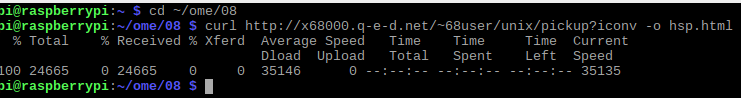
\includegraphics[width=\textwidth]{./text08-img/textbook-img020.png}

\end{center}

\bigskip

\clearpage
lessで開いてみよう

less hsp.html



\begin{center}
  % Unhandled or unsupported graphics:
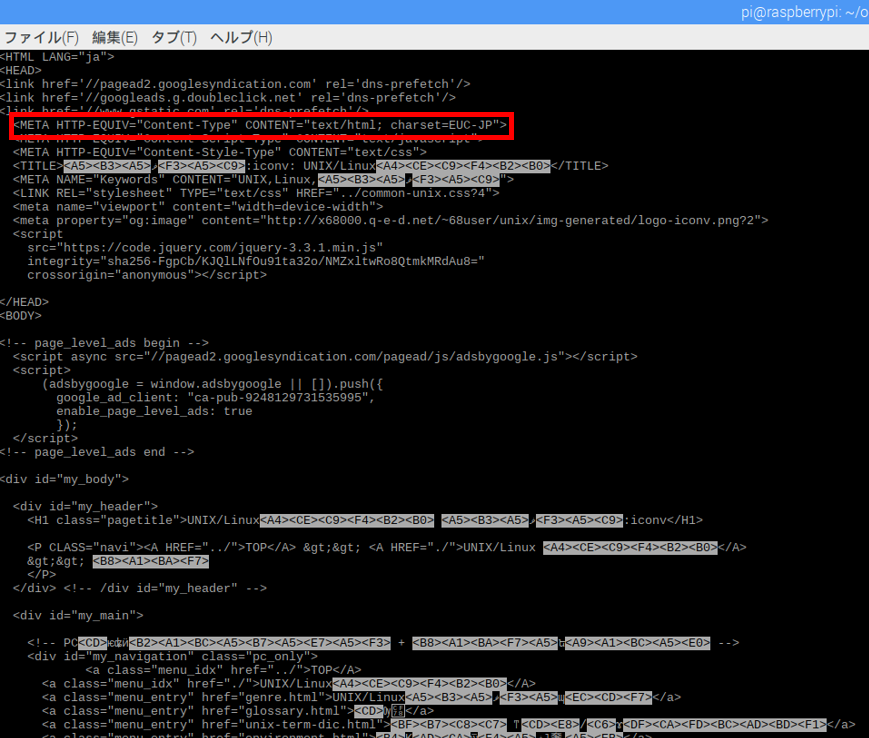
\includegraphics[width=\textwidth]{./text08-img/textbook-img021-1.png}

\end{center}
{\textless}meta
charset=”EUC-JP”{\textgreater}という行を探してみよう。

{\textless}head{\textgreater}{\textless}/head{\textgreater}タグの中に入っているので、先頭のほうにあります。

このHTMLファイルはEUC-JPという文字コードが使われています。

ファイルの中を見てみると、文字化けしている\ruby{箇所}{かしょ}があります。



\begin{center}
  % Unhandled or unsupported graphics:
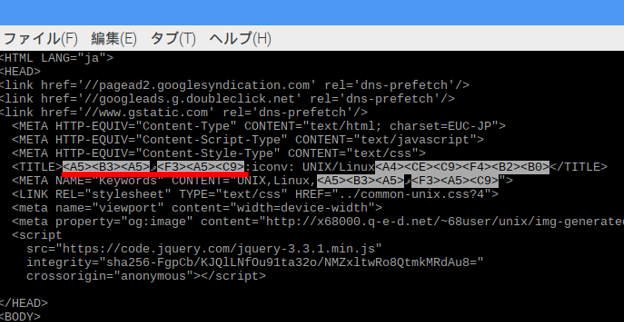
\includegraphics[width=\textwidth]{./text08-img/textbook-img021-2.png}

\end{center}
UTF-8を使っているターミナルへEUC-JPで\ruby{記述}{きじゅつ}されたファイルの中身を表示したので、このように文字化けしてしまいます。


\bigskip

\refstepcounter{Exercise}
% \clearpage\section{\theExercise ウェブページで使用されている文字コードを変換する}
\clearpage\section{\theExercise iconvで文字コードを指定してみよう}
\addtocounter{Exercise}{-1}\refstepcounter{Exercise}\label{E:iconv2}

文字化けを解消するために、EUC-JPからUTF-8へ変換してみよう

\textbf{iconv hsp.html -f EUC-JP -t UTF-8 -o hsp\_utf8.html}

% \begin{center}
% \begin{boxedminipage}{17.228cm}
% \section*{コラム
% iconvコマンドのオプション(機能)}
% iconvのオプションについて

% {}-fオプションでは変換前の文字コードを指定します。

% {}-tオプションでは変換後の文字コードを指定します

% {}-oオプションはcurlと同じで、出力ファイル名を指定します。

% iconv hsp.html -f EUC-JP -t UTF-8 -o hsp\_utf8.html

% では、hsp.htmlをEUC-JPからUTF-8に変換してhsp\_utf8.htmlとして出力するという意味になります。
% \end{boxedminipage}
% \end{center}


\begin{table}[htbp]
    \centering
    % \caption{文字タイプ表}
    \begin{tabular}{|l|}
        \hline
        コラム iconvコマンドのオプション(機能) \\
        iconvのオプションについて\\

        {}-fオプションでは変換前の文字コードを指定します。\\

        {}-tオプションでは変換後の文字コードを指定します\\

        {}-oオプションはcurlと同じで、出力ファイル名を指定します。\\

        iconv hsp.html -f EUC-JP -t UTF-8 -o hsp\_utf8.html\\

        では、hsp.htmlをEUC-JPからUTF-8に変換してhsp\_utf8.htmlとして出力するという意味\\
        になります。\\
        \\\hline
    \end{tabular}
\end{table}






\begin{center}
  % Unhandled or unsupported graphics:
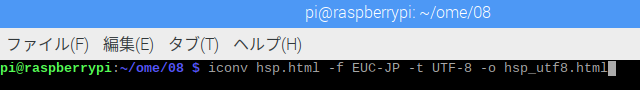
\includegraphics[width=\textwidth]{./text08-img/textbook-img022.png}

\end{center}

\clearpage

変換ができたら、同様にlessコマンドで見てみよう

\textbf{less hsp\_utf8.html}



\begin{center}
  % Unhandled or unsupported graphics:
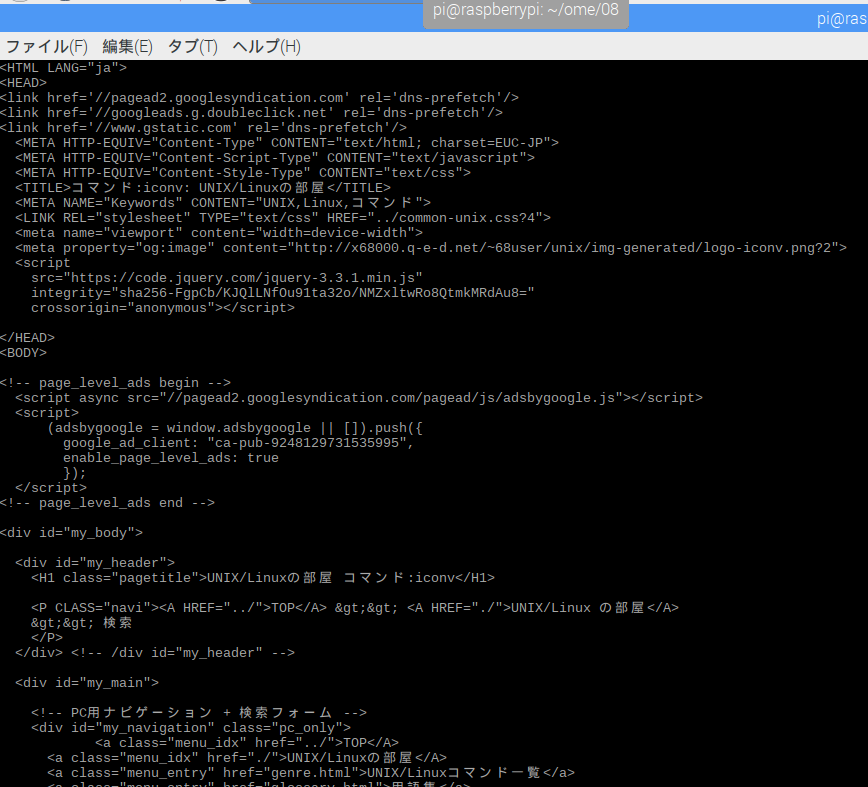
\includegraphics[width=\textwidth]{./text08-img/textbook-img023.png}

\end{center}
変換したファイルでは文字化けはしていません。
文字コードの変換ができました。

\clearpage
しかし、HTMLファイルは{\textless}meta
charset=””{\textgreater}で文字コードを指定しています。
ブラウザやHTMLを扱うソフトウェアの多くはここに書かれている文字コードを使用してHTMLを理解します。

試しに、UTF-8に変換したHTMLファイル\textbf{({\textasciitilde}/08/hsp\_utf8.html)}をブラウザで開いてみよう。

ブラウザを開いて、

\textbf{{\textasciitilde}/08/hsp\_utf8.html} と入力しエンターを押します。

\begin{center}
  % Unhandled or unsupported graphics:
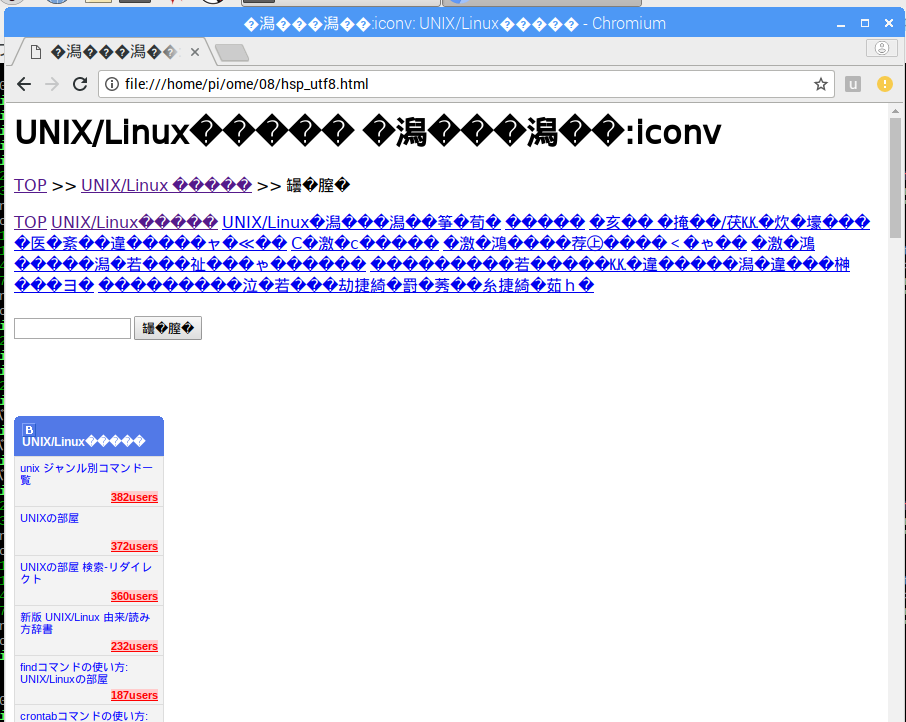
\includegraphics[width=0.95\textwidth]{./text08-img/textbook-img024.png}

\end{center}
表示されているほとんどが、文字化けしています。
\ruby{画像}{がぞう}はダウンロードしていないので表示されません。
これは、ファイルの中身をUTF-8に変換したけれど、ブラウザやHTMLを扱う多くのソフトウェアは{\textless}meta
charset=””{\textgreater}を確認して文字コードを\ruby{判断}{はんだん}します。
ここを\ruby{修正}{しゅせい}しなければ、正しく扱われません。
このタグで指定している文字コードを変換後の文字コードであるUTF-8に変更して置く必要があります。



\refstepcounter{Exercise}
% \clearpage\section{\theExercise ウェブページで使用されている文字コードを変換する}
\clearpage\section{\theExercise mousepadから文字コードを指定してみよう}
\addtocounter{Exercise}{-1}\refstepcounter{Exercise}\label{E:iconv3}

ターミナルで、

mousepadと入力し、実行してmousepadを開きましょう。



\begin{center}
  % Unhandled or unsupported graphics:
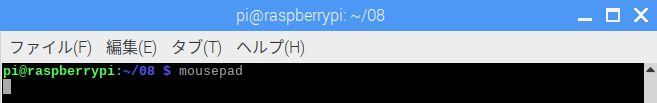
\includegraphics[width=\textwidth]{./text08-img/textbook-img006.png}

\end{center}

% 続いて、mousepadの

% ファイル→ 開くから

% hsp\_utf8.htmlをクリックし、開きます。


続いて、mousepadの
ファイル→開く
をクリックし、hsp\_utf8.html を開きます。


charset=”EUC-JP”を探して、



\begin{center}
  % Unhandled or unsupported graphics:
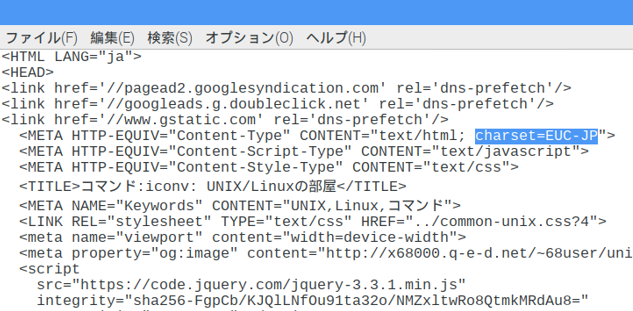
\includegraphics[width=\textwidth]{./text08-img/textbook-img025.png}

\end{center}
charset=”UTF-8”に変更します。



\begin{center}
  % Unhandled or unsupported graphics:
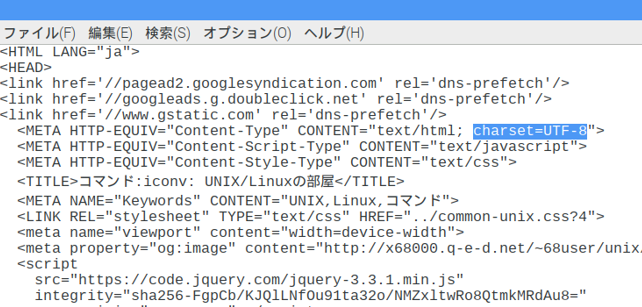
\includegraphics[width=\textwidth]{./text08-img/textbook-img026.png}

\end{center}

\clearpage

保存してブラウザをリロードすると



\begin{center}
  % Unhandled or unsupported graphics:
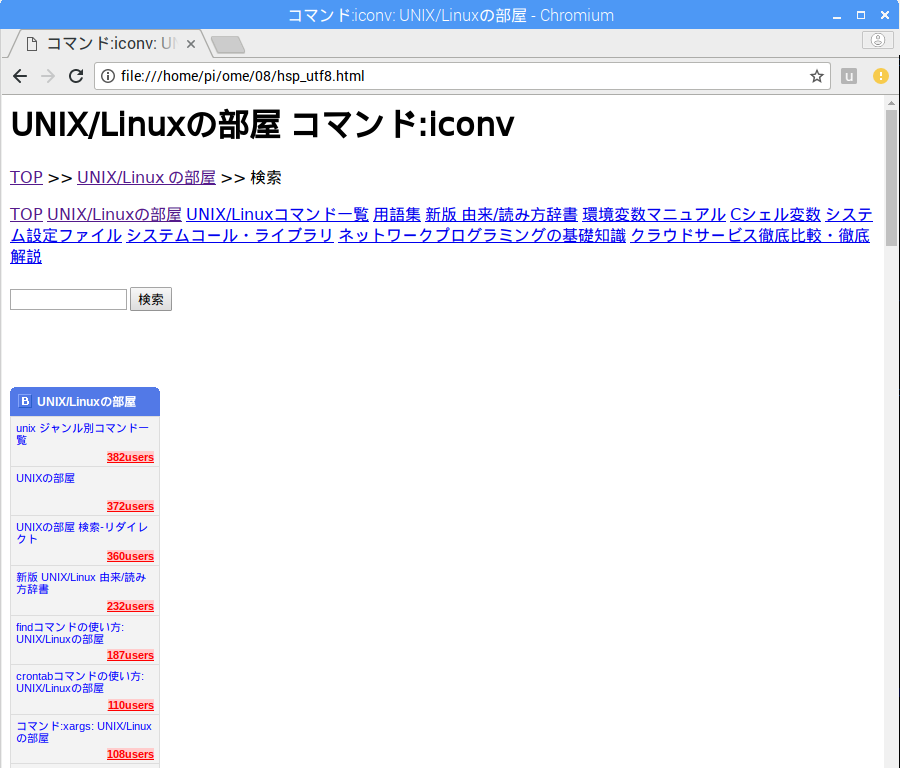
\includegraphics[width=0.95\textwidth]{./text08-img/textbook-img027.png}

\end{center}


\bigskip


\bigskip

文字化けせずに正しく表示されました。
HTMLファイルの文字コードを変換するときは、{\textless}meta
charset=””{\textgreater}を変換後の文字コードに変更するのを\ruby{忘}{わす}れないようにしましょう。
